\chapter{Requisitos Funcionais}
\minitoc
\section{Âmbito do projecto}
\subsection{Situação actual}
Actualmente, o mercado de segurança em redes informáticas disponibiliza uma grande variedade de sistemas de segurança, sob vários pontos de vista.
Estes sistemas podem tomar a forma de sistemas de prevenção a ataques a uma rede com serviços, protecção contra ataques, através da
escrita de regras de acesso à rede e ainda análise de ataques.\\
Todos estes serviços/produtos geram informação que é necessário que é lida pelo administrador de rede, afim de compreender o tipo de ataque que houve,
se o sistema de protecção foi eficaz e se não, tentar melhorar o sistema em causa.\\
Muitas fezes estes sistemas geram ficheiros de log muito grandes e practicamente complexos para um humano interpretar e extraír informação.\\
Suprir esta lacuna é o mote para o desenvolvimento deste produto que deverá mostrar através de uma forma clara os ataques que uma rede foi alvo
e ainda os ataques que o honeypot sofreu. Por forma a que o administrador de rede compreenda facilmente e na totalidade o tipo de ataque que a sua rede sofreu.
Com esta informação espera-se que a tarefa de melhorar a segurança de rede seja facilitada ao administrador.

\subsection{Contexto do projecto}
Por forma a dar uma melhor ideia geral da arquitectura do projecto e por forma a mostrar de que forma a compreender
a interacção das várias entidades do sistema (quer sejam humanas ou não) é imperativo que se modele um diagrama de contexto.
Neste diagrama iremos mostrar quais as entidades externas ao sistema informático que vão ter algum relacionamento com este, 
isto é, quais as actividades que o sistema informático vai suportar no negócio em questão. 

\subsection{Diagrama de Contexto}
Para explicar com maior detalhe o sistema de que estamos a falar mostramos na Figura \ref{fig:dcont} o diagrama de contexto.

\begin{figure}[!ht]
\centering
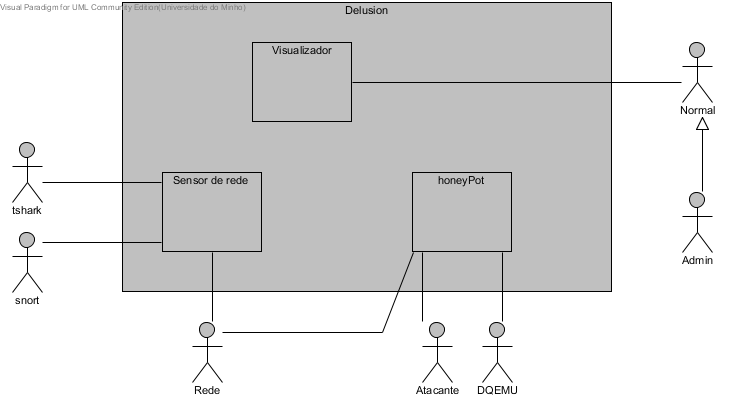
\includegraphics[scale=0.8]{images/DiagramaContexto}
\caption{Diagrama de Contexto}
\label{fig:dcont}
\end{figure}

Como se pode ver nesse diagrama apresentamos os três elementos mais importantes deste projecto, o Visualizador, o Sensor de rede e o Honeypot.
O Visualizador apresenta uma interface web para o utilizador deste sistema, o Sensor de rede usa como entidades externas duas ferramentas para fazer inspecção
ao nível de rede: o tshark e o snort. Ainda temos o componente de Honeypot que usa o DQEMU (a ferramenta que vamos desenvolver), este sistema tem ainda
como actor o atacante, pois este irá ser atraído para este sistema e será gravada toda a sua actividade dentro do Honeypot.\\
Existem dois tipos de utilizadores do Visualizador: O utilizador Admin que tem total controlo sobre o sistema, podendo ler informação sobre os ataques, bem como
criar novos honeypots na rede com determinadas caracteristicas. Temos ainda o utilizador Normal que terá os mesmos privilégios que o Admin, mas apenas num
segmento menor da rede, segmento esse que será o Admin a atribuir.


